\newpage
\usecaseautenticato{Visualizzazione notifica nuovo messaggio in \textit{chat}}
\label{usecase:Visualizzazione notifica nuovo messaggio in chat}

\begin{figure}[h]
	\centering
	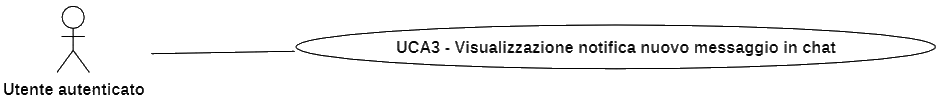
\includegraphics[width=0.9\textwidth]{./uml/UCA3.png} 
	\caption{Visualizzazione notifica nuovo messaggio in \textit{chat}}
	\label{fig:UCA3}
  \end{figure}

\begin{itemize}
    \item \textbf{Attore principale:} Utente autenticato.
	
	\item \textbf{Precondizione:} L'Utente base oppure l'Utente ristoratore ha inviato un messaggio in \textit{chat} (vedi \autoref{usecase:Invio messaggio chat}).

	\item \textbf{Postcondizione:} L'Utente autenticato destinatario del messaggio visualizza la notifica della presenza di un nuovo messaggio in \textit{chat}.
     
	\item \textbf{Scenario principale:}
	      \begin{enumerate}
                \item L'utente invia un messaggio;
                \item Il Sistema vede che al suo interno è stato memorizzato un nuovo messaggio;
                \item Il Sistema invia al destinatario la notifica di ricezione di un nuovo messaggio;
                \item L'Utente autenticato destinatario del messaggio visualizza la notifica della presenza di un nuovo messaggio in \textit{chat}.
	      \end{enumerate}
\end{itemize}